\documentclass[cropped,10pt]{standalone}

\usepackage{tikz}

% helvetica font
\usepackage[scaled=1.1]{helvet}
\usepackage{sfmath}
\renewcommand{\familydefault}{\sfdefault}

% or comment out previous 3 lines, and uncomment the one below, for clean latex font
%\usepackage{cmbright}

% you might want to define some colors:
%\definecolor{myred}{HTML}{E51E10}
%\definecolor{myblue}{HTML}{56B4E9}

\usetikzlibrary[positioning,arrows,arrows.meta,shapes,calc,spy,intersections,shadows,bending]
\usetikzlibrary[decorations.text,decorations.pathmorphing,decorations.markings]

\pagestyle{empty}
\thispagestyle{empty}

\begin{document}

\begin{tikzpicture}

% ----------------------------------------------------

% helper grid (comment out once you're done!)
%\draw[help lines,step=1,thin,gray!20] (0,0) grid (100, 100);
%\draw[help lines,step=5,gray!20,very thick] (0,0) grid (100, 100);
%\draw[help lines,step=10,gray!40,ultra thick] (0,0) grid (100, 100);
%
%\foreach \j in {10,15,..., 50}
%  \node at (\j,85) [fill=white,text=red!80!black] {\j};
%\foreach \j in {10,15,..., 95}
%  \node at (23,\j) [fill=white,text=green!80!black] {\j};
%
% ----------------------------------------------------

  \node at (0, 99) [anchor = north west] {
  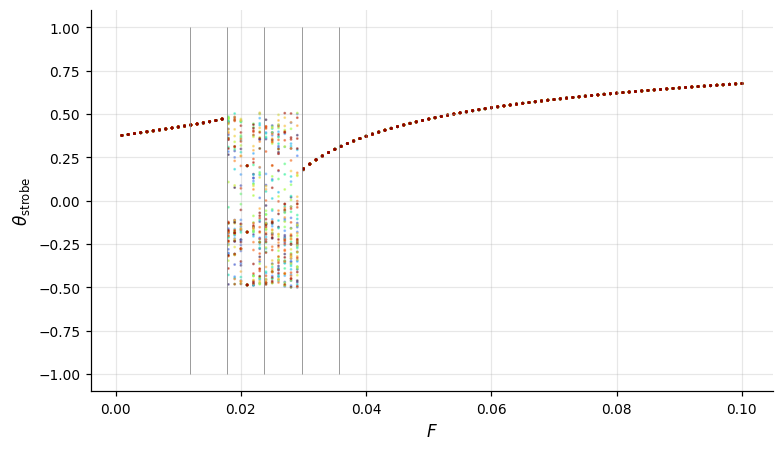
\includegraphics{../figures_melnikov/figure_bif_duff.png}
  };
  \node at (18, 99) [anchor = north west] {
  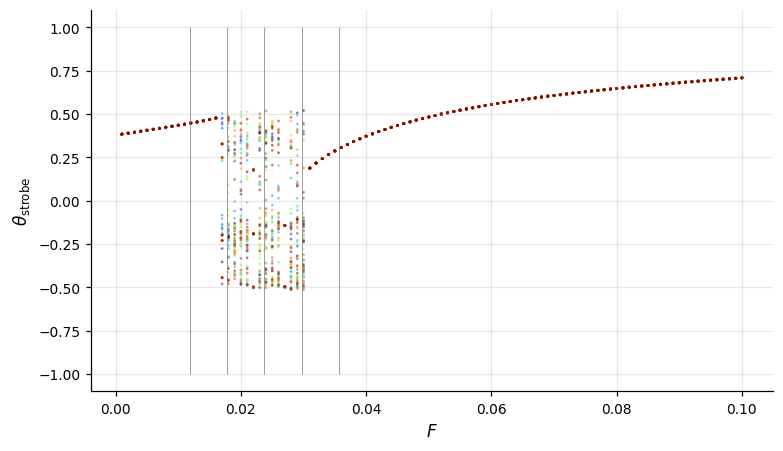
\includegraphics{../figures_melnikov/figure_bif_bessel.png}
  };
  \node at (0, 88) [anchor = north west] {
  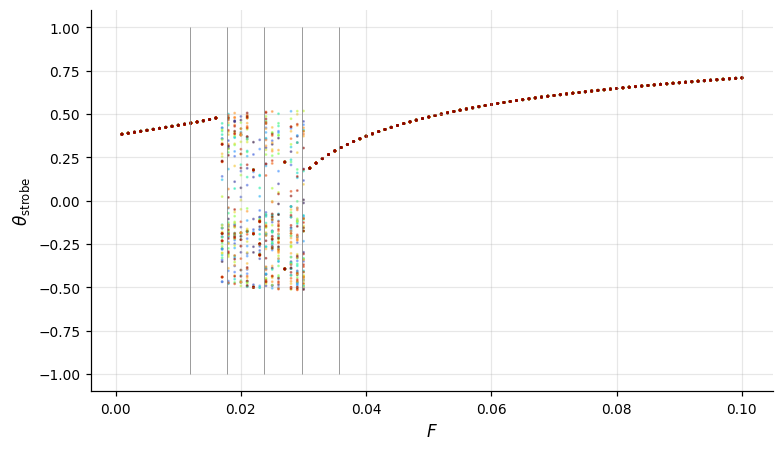
\includegraphics{../figures_melnikov/figure_bif_pfl3.png}
  };
  \node at (18, 88) [anchor = north west] {
  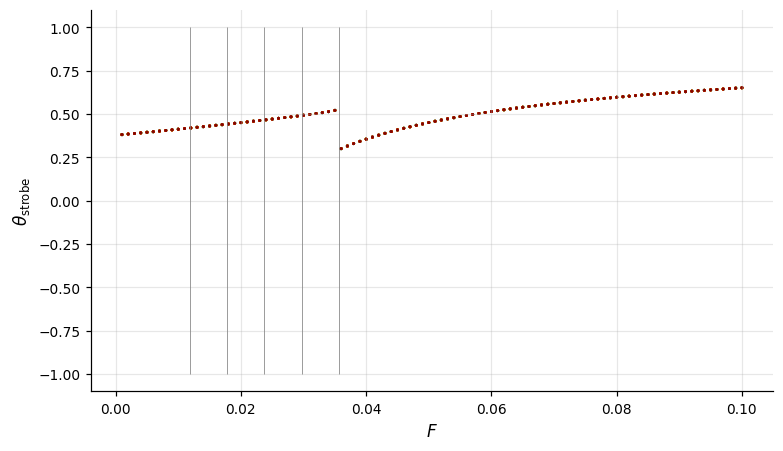
\includegraphics{../figures_melnikov/figure_bif_fc.png}
  };
  \node at(0, 100)[anchor = north, font = \bfseries, scale = 3]{A};
  \node at(18, 100)[anchor = north, font = \bfseries, scale = 3]{B};
  \node at(0, 89)[anchor = north, font = \bfseries, scale = 3]{C};
  \node at(18, 89)[anchor = north, font = \bfseries, scale = 3]{D};

% HERE YOU CAN USE TIKZ CODE TO ADD DIAGRAMS ETC

% don't forget all your panel labels etc
% e.g.:
% \node at (10,90) [anchor=base,font=\bfseries,scale=1.5] {A};

\end{tikzpicture}
\end{document}

